\chapter{Cwiczenie 1 - Czwórnik CR}

\newcommand{\Ra}{49,4}
\newcommand{\Rb}{3,9k}
\newcommand{\Rc}{1,545k}
\newcommand{\C}{209,6nF}

\section{Polecenie}
Należało zmontować \textbf{czwórnik CR} oraz zmierzyć jego charakterystyki częstotliwościowe amplitudy i fazy. Na podstawie zmierzonych wartości należało wyznaczyć dolną częstotliwość graniczną oraz porównać z wyliczoną wartością teoretyczną.

\section{Dobór oporników}

\begin{itemize}
    \begin{figure}[h]
        \centering
        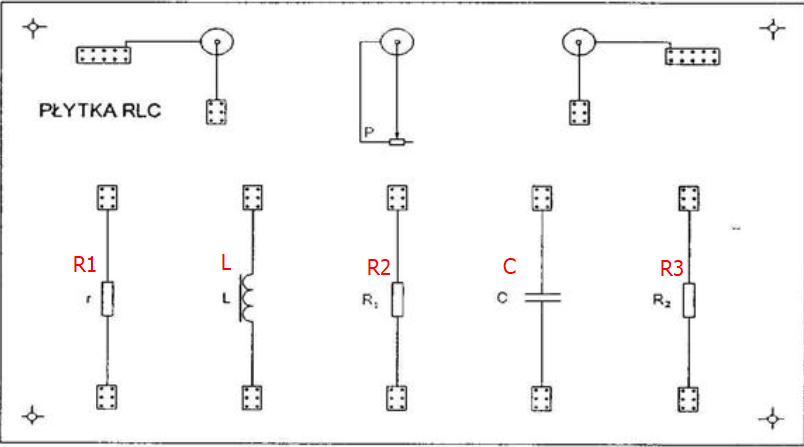
\includegraphics[scale=0.7]{img_wyklad/Schemat_plytki_RLC.png}
        \caption{Schemat używanej płytki RLC}
        \label{fig:schemat_plytki_RLC}
    \end{figure}
    \item Zmierzono wartości rezystorów oraz kondensatora za pomocą multimetra:
        \begin{center}
            \textbf{R1 = \Ra}\boldsymbol{\Omega} \\
            \textbf{R2 = \Rb}\boldsymbol{\Omega} \\
            \textbf{R3 = \Rc}\boldsymbol{\Omega} \\
            \textbf{C = \C}
        \end{center}
    \item Dobrano stałą czasową $\tau$ tak, aby była ona z przedziału 0,1 - 1 ms.
        \begin{gather}
           \tau_1 = R_1 \cdot C = \Ra\Omega \cdot \C \approx 1,03 \cdot 10^{-5}s \\
           \tau_2 = R_2 \cdot C = \Rb\Omega \cdot \C \approx 0.8 \cdot 10^{-3}s \\
           \tau_3 = R_3 \cdot C = \Rc\Omega \cdot \C \approx 0,32 \cdot 10^{-3}s
        \end{gather}
    \newpage
    \item Zmontowano układ używając opornika\textbf{ R2 = \Rb}$\boldsymbol{\Omega}$, posługując się trójnikiem rozdzielono wejście tak, aby na oscyloskopie można było obserwować sygnał wejściowy oraz wyjściowy:
    \begin{figure}[h]
        \centering
        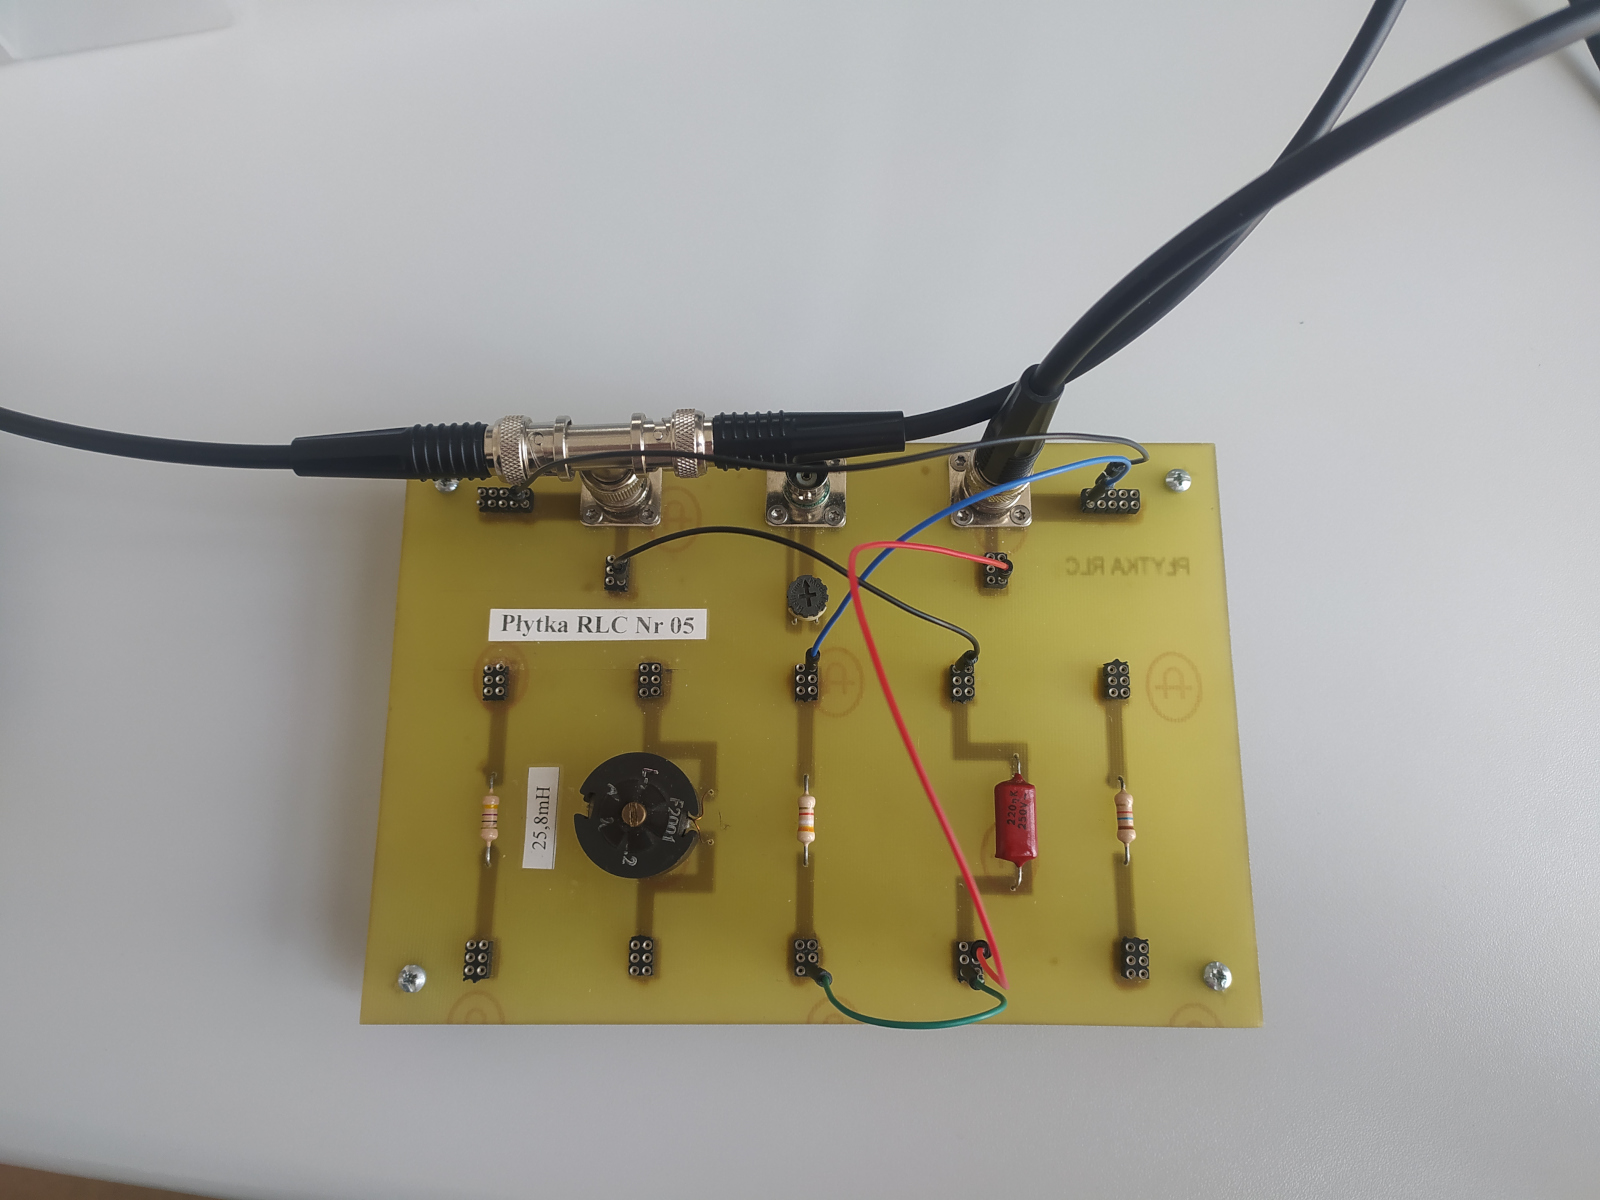
\includegraphics[scale=0.15]{img_phone/IMG_20220330_094222_smaller.jpg}
        \caption{Zmontowany czwórnik CR}
        \label{fig:builtCR}
    \end{figure}
\end{itemize}

\begin{itemize}    
    \item Dokonano wstępnego pomiaru wysyłając z generatora funkcyjnego sygnał o amplitudzie \textbf{1V}.
    \label{literowka:oscylator} \item \textcolor{purple}{Oscyloskop} wskazał błędną wartość amplitudy = \textbf{2V}
\end{itemize}

\begin{figure}[h]
    \centering
    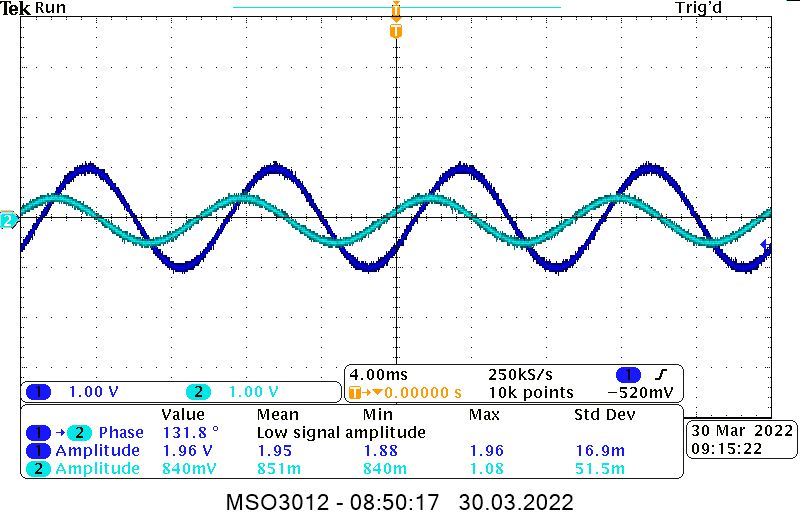
\includegraphics[scale=0.4]{img_osciloscope/2_sinusy_zzla_amplituda_cropped.png}
    \caption{Zły pomiar}
    \label{fig:zly_pomiar}
    \end{figure}

\begin{itemize}
    \item Poprawiono ustawienia na generatorze funkcyjnym.
        \begin{center}
            \textbf{Output Menu $\xrightarrow{}$ Load Impedance $\xrightarrow{}$ High Z.}
        \end{center}
    \item Przystąpiono do badania charakterystyk częstotliwościowych.
\end{itemize}

\newpage

\section{Pomiary}

\begin{itemize}
    \item Wyliczono początkową wartość, z której zaczęto mierzyć charakterystykę:
        \begin{equation}
            f_0 = \frac{1}{\tau} = \frac{1}{0.8 * 10^{-3}s} = 1.25 * 10^3 \frac{1}{s} = 1.25kHz
        \end{equation}
    \item Przesyłano sygnał o amplitudzie \textbf{2V} oraz częstotliwościach z przedziału $\langle\textbf{25};\textbf{1000}\rangle$, pomiary pobierane zostały za pomocą funkcji wbudowanych w oscyloskopie. \\
    \textbf{1 kanał - wejście} \\
    \textbf{2 kanał - wyjście}
\end{itemize}

\begin{itemize}
    \item \textcolor{purple}{Zmierzone wartości w postaci tabeli}:
\begin{center}
    \Large %tabelka Uwe Uwy phi
    \label{poprawa:pomiary_CR}
    \begin{tabular}{|>{\columncolor[gray]{0.8}}c|>{\columncolor[gray]{0.8}}c|c|>{\columncolor[gray]{0.8}}c|c|}
         \hline
         $f$ [Hz] & $U_{we}$ [V] & $U_{wy}$ [V] & $\frac{U_{wy}}{U_{we}}$ & $\phi$ [$\degree$] \\
         \hline
         25 & 1.98 & 0.252 & 0.127 & -82.5 \\
         \hline
         50.03 & 1.98 & 0.499 & 0.252 & -75.59 \\
         \hline
         100.1 & 1.98 & 0.895 & 0.452 & -63.42 \\
         \hline
         198.8 & 1.98 & 1.4 & 0.7 & -45.62 \\
         \hline
         300 & 1.98 & 1.64 & 0.82 & -34.10 \\
         \hline
         464.8 & 1.98 & 1.8 & 0.9 & -22.98 \\
         \hline
         545,5 & 1.98 & 1.85 & 0.93 & -20.27 \\
         \hline
         622 & 1.98 & 1.88 & 0.94 & -18.87 \\
         \hline
         699.5 & 1.98 & 1.9 & 0.95 & -15.35 \\
         \hline
         799.7 & 1.98 & 1.91 & 0.964 & -13.4 \\
         \hline
         856 & 1.98 & 1.92 & 0.969 & -12.71 \\
         \hline
         1000 & 1.98 & 1.92 & 0.969 & -12.33 \\
         \hline
    \end{tabular}
\end{center}

    \item Poniżej zostały przedstawione zrzuty wyświetlacza z oscyloskopu przeprowadzonych pomiarów:
%osciloscope_figures 
    {
    \begin{figure}[H]
        \centering
        \begin{subfigure}[h]{0.45\textwidth}
            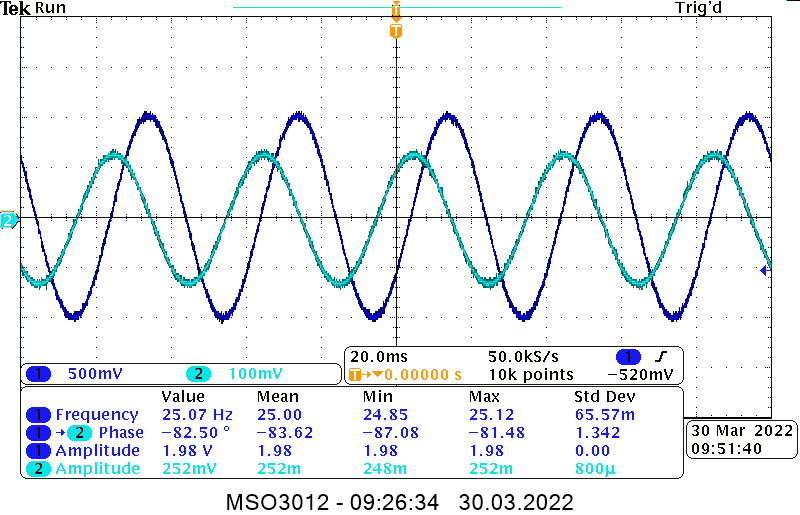
\includegraphics[width=\textwidth]{img_osciloscope/CR/CR_25Hz_cropped.png}
            \caption*{25Hz}
        \end{subfigure}
        \begin{subfigure}[h]{0.45\textwidth}
            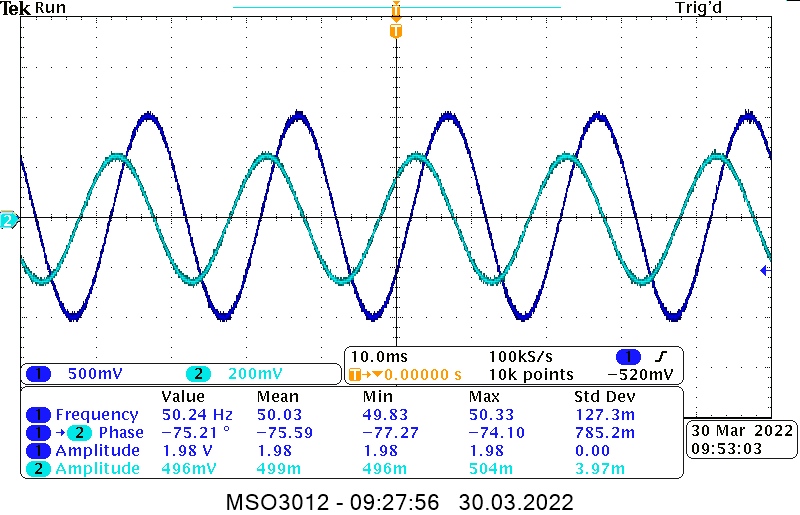
\includegraphics[width=\textwidth]{img_osciloscope/CR/CR_50Hz_differentscale_cropped.png}
            \caption*{50Hz}
        \end{subfigure}
    \end{figure}
    
    \begin{figure}[H]
        \centering    
        \begin{subfigure}[h]{0.4\textwidth}
            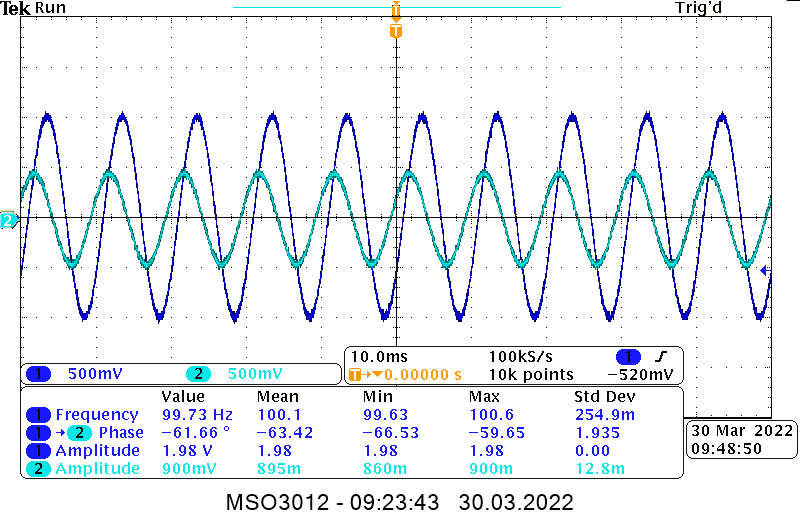
\includegraphics[width=\textwidth]{img_osciloscope/CR/CR_100Hz_cropped.png}
            \caption*{100Hz}
        \end{subfigure}
        \begin{subfigure}[h]{0.4\textwidth}
            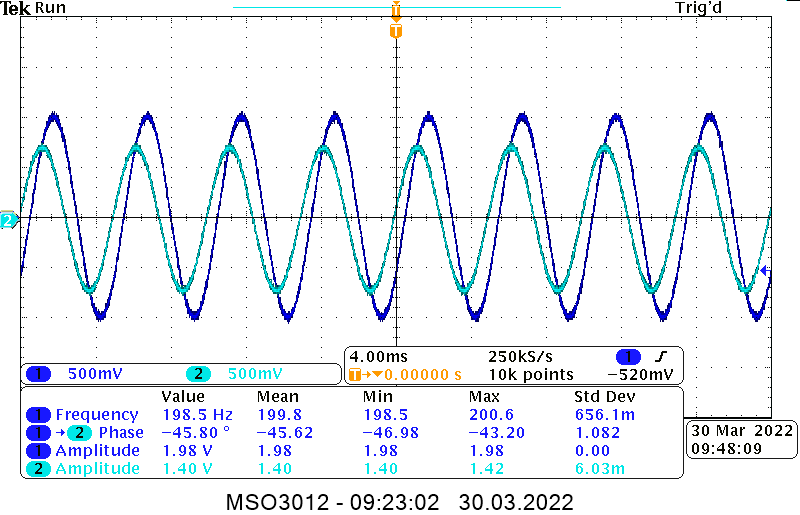
\includegraphics[width=\textwidth]{img_osciloscope/CR/CR_200Hz_cropped.png}
            \caption*{200Hz}
        \end{subfigure}
    \end{figure}
    
    \begin{figure}[H]
        \centering
        \begin{subfigure}[h]{0.4\textwidth}
            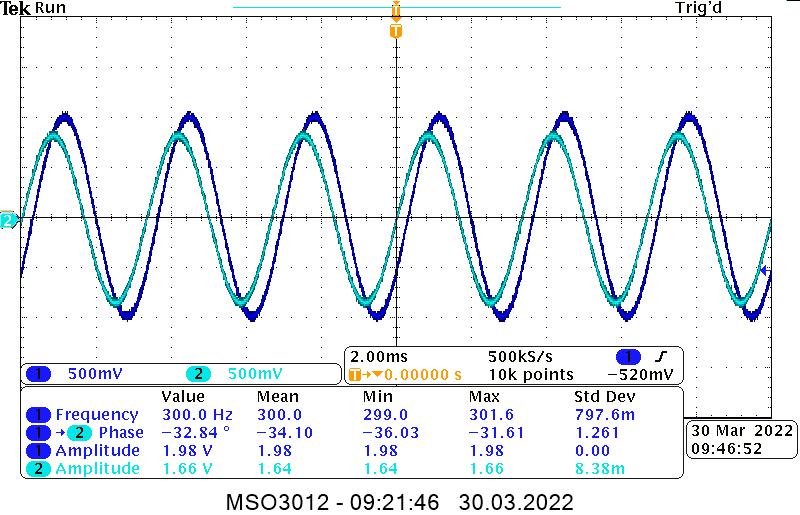
\includegraphics[width=\textwidth]{img_osciloscope/CR/CR_300Hz_cropped.png}
            \caption*{300Hz}
        \end{subfigure}
        \begin{subfigure}[h]{0.4\textwidth}
            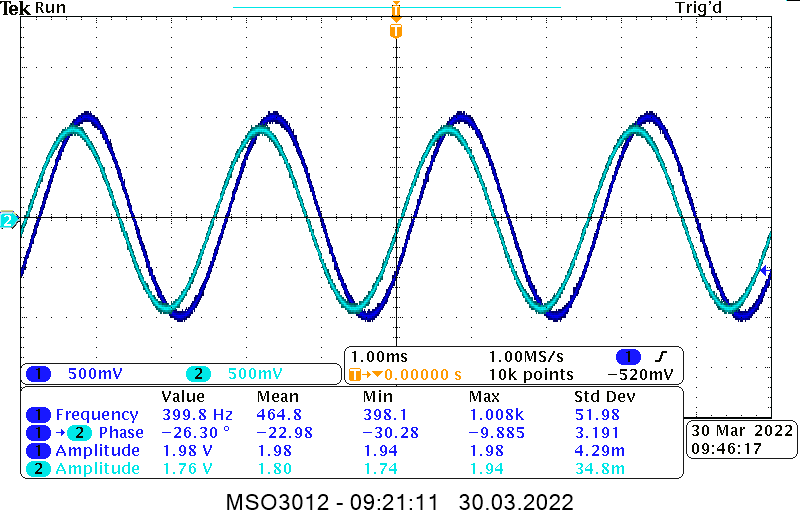
\includegraphics[width=\textwidth]{img_osciloscope/CR/CR_400Hz_cropped.png}
            \caption*{400Hz}
        \end{subfigure}
    \end{figure}
    
    \begin{figure}[H]
        \centering
        \begin{subfigure}[h]{0.4\textwidth}
            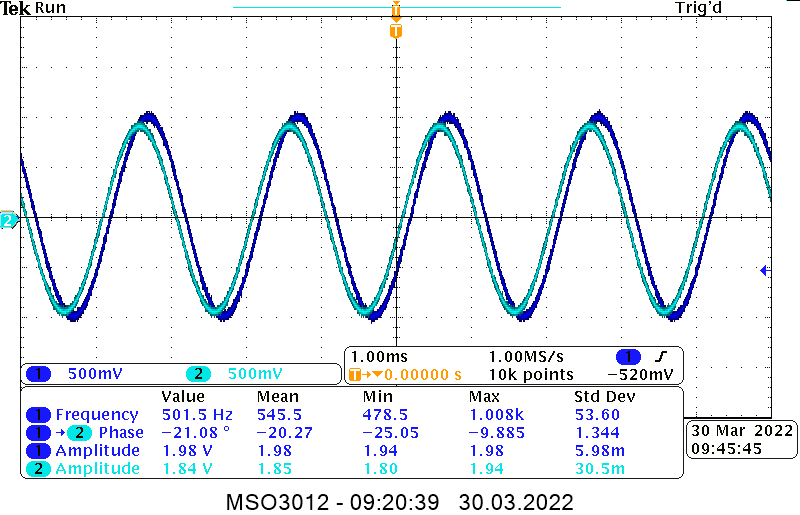
\includegraphics[width=\textwidth]{img_osciloscope/CR/CR_500Hz_cropped.png}
            \caption*{500Hz}
        \end{subfigure}
        \begin{subfigure}[h]{0.4\textwidth}
            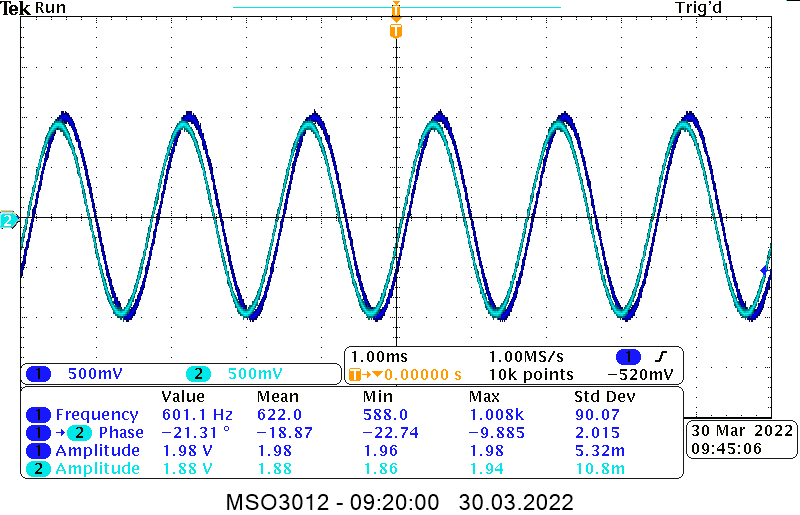
\includegraphics[width=\textwidth]{img_osciloscope/CR/CR_600Hz_cropped.png}
            \caption*{600Hz}
        \end{subfigure}
    \end{figure}
    
    \begin{figure}[H]
        \centering
        \begin{subfigure}[h]{0.4\textwidth}
            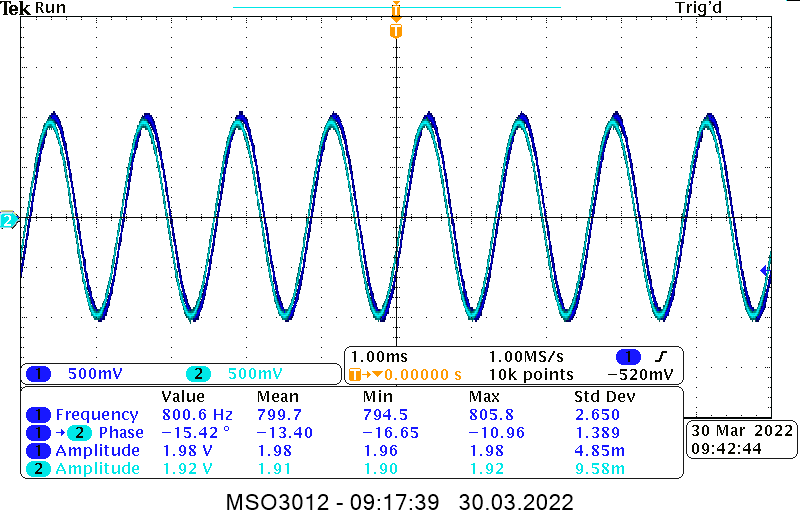
\includegraphics[width=\textwidth]{img_osciloscope/CR/CR_800Hz_cropped.png}
            \caption*{800Hz}
        \end{subfigure}
        \begin{subfigure}[h]{0.4\textwidth}
            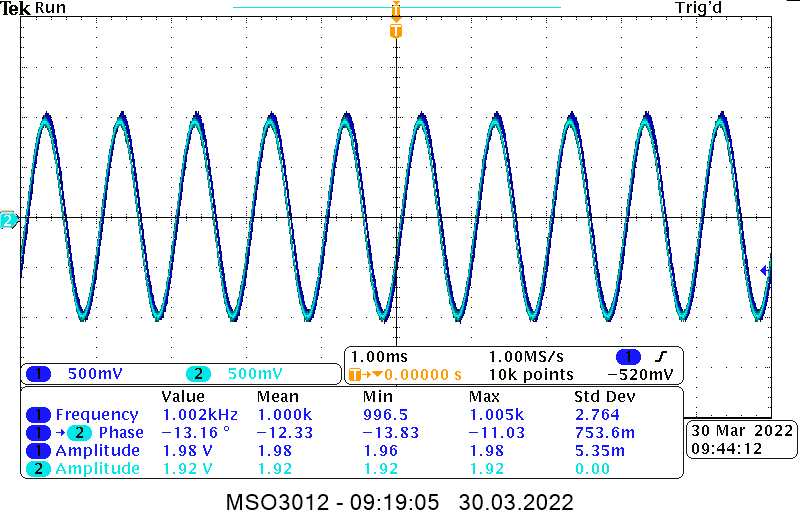
\includegraphics[width=\textwidth]{img_osciloscope/CR/CR_1000Hz_cropped.png}
            \caption*{1000Hz}
        \end{subfigure}
    \end{figure}
    }
\end{itemize}

\newpage
\section{Charakterystyka amplitudowa}
    \begin{itemize}
        \item Stałe:
            \begin{gather}
                \tau = RC = 0.8 * 10^{-3}s \\
                \omega_0 = \frac{1}{RC} = \frac{1}{\tau}
            \end{gather}
        \item Funkcja przejścia:
            \begin{equation}
                T(\omega) = \frac{Z_2}{Z_1+Z_2} = \frac{R}{\frac{1}{j \omega C}+R} = \frac{j\frac{\omega}{\omega_0}}{1 + j \frac{\omega}{\omega_0}}
                \label{eqn:f_przejscia}
            \end{equation}
        \item Charakterystyka amplitudowa:
            \begin{equation}
                |T(\omega)| = \sqrt{\frac{(\frac{\omega}{\omega_0})^2}{1 + (\frac{\omega}{\omega_0})^2}}
                \label{eqn:char_amp}
            \end{equation}
        \item Dolna częstotliwość graniczna teoretyczna wyniosła:
            \begin{equation}
                f_t = \frac{1}{2 \pi \tau} \approx \textbf{198.94Hz}
            \end{equation}
        \item Dolna częstotliwość graniczna eksperymentalna wyniosła:
            \begin{equation}
                f_e \approx \textbf{203,4Hz}
            \end{equation}
        \item Różnica między wartością eksperymentalną a teoretyczną wyniosła $\boldsymbol{\Delta}$ = \textbf{4.46Hz} \\
            Funkcja zgadza się z teoretyczną. \\
            Pomiar został uznany za poprawny.
        \begin{figure}[H]
            \centering
            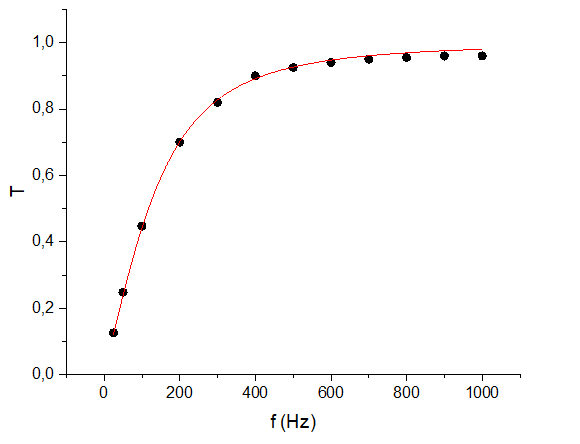
\includegraphics[scale=0.7]{img_wykresy/amplitudowa_CR.png}
            \caption{Charakterystyka amplitudowa | $\bullet$ - punkty eksperymentalne}
            \label{fig:CR_amp}
        \end{figure}
    \end{itemize}

\section{Charakterystyka fazowa}

\begin{itemize}
    \item Stałe:
    \begin{gather}
        \tau = RC = 0.8 * 10^{-3}s \\
        \omega_0 = \frac{1}{RC} = \frac{1}{\tau}
    \end{gather}
    \item Funkcja przejścia wynosi:
        \begin{equation}
            T(\omega) = \frac{(\frac{\omega}{\omega_0})^2 + j\frac{\omega}{\omega_0}}{1 + (\frac{\omega}{\omega_0})^2}
        \end{equation}
    \item Charakterystyka fazowa:
        \begin{equation}
            \phi(\omega) = \arctan({\frac{Im T(\omega)}{Re T(\omega)}}) = \arctan({\frac{\omega_0}{\omega}})
        \end{equation}
    \item Dolna częstotliwość teoretyczna wyniosła: 
        \begin{equation}
            f_t = \frac{1}{2\cdot\pi\cdot\tau} \approx \textbf{198.94Hz}
        \end{equation}
    \item Dolna częstotliwość eksperymentalna wyniosła:
        \begin{equation}
            f_e \approx \textbf{195,77Hz}
        \end{equation}
    \item Różnica między wartością eksperymentalną a teoretyczną wyniosła $\boldsymbol{\Delta}$ = \textbf{3.17Hz} \\
        Funkcja zgadza się z teoretyczną. Pomiar został uznany za poprawny.
    \begin{figure}[H]
        \centering
        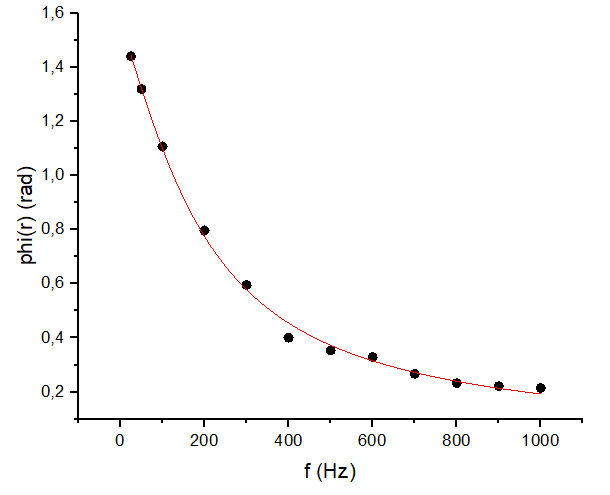
\includegraphics[scale=0.6]{img_wykresy/fazowa_CR.png}
        \caption{Charakterystyka fazowa | $\bullet$ - punkty eksperymentalne}
        \label{fig:CR_amp}
    \end{figure}
\end{itemize}